Bluetooth is a wireless communication technology created in 1994 by the mobile telecommunication company Ericsson. Bluetooth was designed for low-power consumption devices such as sensors, mobile phones, etc. Nowadays, more and more devices use Bluetooth mainly due to the uprising of Internet of Things (IoT) and small battery reliant devices.

\subsubsection{Bluetooth communication}
Bluetooth operates in the 2.4 GHz frequency band and uses frequency-hopping spread spectrum. This FHSS means that each packets from a Bluetooth communication is transmitted on one of 79 channels having a bandwidth of 1MHz each.\\
Bluetooth is also using adaptive frequency-hopping spectrum (AFH), used to avoid crowded frequency in the channel spectrum.\\

In order to fully understand Bluetooth technology, older versions need to be described. The difference between versions were based on the \textit{"versions differences" from links} [XXX] and \textit{Wikipedia}[XXX].\\
In versions 1.X (released between 1994 and 2005), the transmissions could go to a speed up to a theoretical value of 1Mbps. Flow control and retransmission modes for the Logical link control and adaptation protocol (L2CAP) were added in the latest version (v1.2). These versions are now obsolete and nearly extinct.\\
Version 2.0 + EDR (Enhanced Data Rate) was released in 2004, it is the first version implementing this technology, speeding up the maximal data rate transfer to 3Mbps rather than 1Mbps.\\
The version 2.1 + EDR (2007) is not bringing any new speed but despite that, its major improvement is to considerably improve the security of bluetooth. Indeed, SSP (Secure Simple Pairing) is introduced in order to make the pairing process simpler, quicker and safer. More explanations about SSP are given in the next part.\newpage
The case study in this project is however not using this latest version, but the Bluetooth 3.0 + HS (High Speed) which was released in 2009, this version is  the first one providing a high data transfer speed that can go up to 24 Mbit/s. It is able to provide such a speed by using the famous 802.11 wireless protocol, it uses a "go all out" policy which first uses normal Bluetooth communication for pairing process and when a file is wanted to be exchanged or whatsoever,  it swaps to the wireless in order to provide this speed.\\
Currently, the latest version of Bluetooth is 4.1 which is known as Bluetooth Low Energy (BT-LE). As its name says, BT-LE was designed to reduce power consumption while providing the same communication range and speed that were used in the previous versions. This version also is simpler than the 3.0 and uses AES to encrypt data. However, it is less secure due to its simplicity and this version has proven MiTM attacks [XXX].\\
The information provided further in this report about bluetooth technology is concerning the version 3.0+HS, although it may be applicable in other versions as well.

\subsubsection{Device ID}

The Bluetooth address (BD\_ADDR) of a device is composed of 48 bits. \\
This address is divided into three parts, the first one being called the UAP (Upper Address Part) which is 8 bits long and, combined with the second part, the Non-significant Address Part (NAP, 16 bits long), they form together the manufacturer ship, or company\_id. The last part is 24 bits long and is the Lower Address Part (LAP), almost uniquely identifying a device, this one will be used in the first stage of sniffing in order to decode the captured packets (This will be further explained later on). This is shown in the figure 1 below.\\


\begin{figure}[!h]
  \begin{center}
	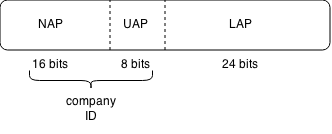
\includegraphics[width=200px]{images/bd_addr.png}
	\label{Bluetooth address}
	\caption{Bluetooth address definition}
  \end{center}
\end{figure}
\newpage
\subsubsection{Overview of Bluetooth security}

The basic security in Bluetooth is set up by the user, he has the choice between three different modes:
\begin{itemize}[nolistsep,noitemsep]
 	\item Silent: In this mode, the device will not initiate any connection. The only thing it does is monitoring the traffic.
 	\item Public: The device is discoverable by anyone around it having its bluetooth activated.
 	\item Private: The device will in that case only answer to device that it already paired with, thus making it (theoretically) only discoverable to known devices.\\
\end{itemize}

\noindent A Bluetooth device can implement four different security modes:

  \begin{itemize}[nolistsep,noitemsep]
  	\item Non Secure: As its name suggests there is no security.
  	\item Service-level enforced security mode: It establishes a non secure ACL (Asynchronous connectionless) link between the two devices willing to communicate. In order to introduce optional encryption, authentication and authorization, a request has to be made via L2CAP (Logical Link Control and Adaptation Protocol) connection-oriented or connection-less channel. This mode is used in versions 2.0 + EDR and below.
  	\item Link level enforced security mode: Once the ACL links are done then security procedures are initiated.
  	\item Service-level enforced security mode: This one is very similar to the second mode except that it introduces SSP (Secure Simple Pairing) and this is compatible only with Bluetooth versions from 2.1 + EDR.
  \end{itemize}

\subsubsection{Pairing process}

As it is briefly explained earlier, SSP has been implemented in order to overcome the weakness of the 4 digits pass at pairing time (only about 10.000 possibilities max) in addition to make the pairing process easier than it used to be. Indeed, using an elaborated Bluetooth sniffer would allow to almost instantly find these digits and then bypassing the security.\\
	
Two devices pair by creating a shared key, called the Link key. This key will be used to authenticate and encrypt the data of two devices.
In order to do so, there are two possibilities: LMP-pairing (4-digits/pincode manner) or SSP. \\
Once this done, the two devices can store their mutual key in order to use it later for a re-pairing, making the connection much faster.\\

In LMP-pairing, the only thing that is not transmitted through the air is the 4 digits PIN code. The pairing process in this case works as follow: \\
The initiator will first generate a 16-bytes random number and then send it to the other device. Once received, both users will put in their PIN code which they will use to create an initialization key, the later will be converted into the actual LMP key. Finally, the two devices have to authenticate each other with their respective newly created LMP key. \\
A software created by Ellisis [XXX] allows an attacker that listens to the traffic to guess with the given information the 4 digits, thus making LMP useless. \\
An overview of the previously explained LMP pairing process is shown in figure 2 below \textit{From ellisys paper in links}: 
\begin{figure}[!h]
  \begin{center}
	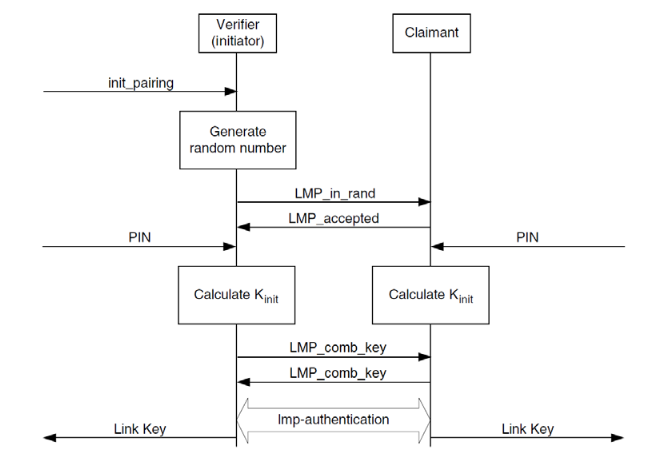
\includegraphics[width=350px]{images/haha.png}
	\label{LMP pairing}
	\caption{LMP pairing process}
  \end{center}
\end{figure}


SSP was then created, fixing the above vulnerability even though it is still possible to find this mechanism in many devices for backward compatibilities. \\
SSP is a new manner of generating a link key (and user numbers such as PIN codes can still be used) using Elliptic Curve in order to create in this situation a much bigger random number now setting the number of possible Link keys to \(2^{128}\) which is far too big to be brute forced, nowadays anyway. 

In order to create a public/private key pair (DHKey), SSP uses the famous Diffie-Hellmann algorithm with a 192-bits random number. The public key is transmitted over the air and can be seen by anyone, the private key is however kept secret for obvious security needs. 

Using two given key pairs A and B, there is a function that allows to result in a DHKey and only the two devices should be able to find it out. This function is F(Public A, Private B)=F(Public B, Private A). This very DHKey will be used in order to create the link key in between the two devices. \\ 
From there, the rest of the pairing process is similar to the LMP-pairing.

\newpage
\textbf{SAFER+ \& Protection against MiTM with SSP}\\

While BTLE uses AES, the older Bluetooth versions up to the 3.0+HS are using SAFER+ (Secure and Fast Encryption Routine) in order to provide authentication and key generation.\\
SAFER+ was candidate to the AES process and like it, it is a family of block ciphers using rounds  and a block size of 128 bits.\\
In bluetooth, SAFER+ is used for key derivation and authentication.\\
This algorithm  uses a non-orthodox linear transformation in order to provide diffusion. It also use additive constant factors in order to avoid weak key generation.\\
Like in AES, it has two main components. The key-scheduling unit which is used in order to provide the round keys on the fly. The second one is called encryption data path, the latter will mix the plaintext with the "feedback" data from the previous rounds.\\


In order to be protected against MiTM attacks, the device can use the user (e.g. to compare two numbers) or Out Of Band (OOB) channel (NFC for example, used to check the integrity of a checksum), these two cases are two of the four association models of SSP. 
Let's define these models:\\
The numeric comparison association model which is the first case above, asking the user to compare numbers.\\
The Passkey Entry association model which is used when one of the device has input capabilities but no displays, in this case only the user with input capabilities will answer the 6-digit pass code.\\
Finally, if one of the device has neither input nor output, and that OOB can't be used, then the JustWork association model is used, which is the weakest model as it simply asks the user to accept the connection.\\
In SSP there are 6 different phases in the pairing process:
\begin{enumerate}[nolistsep,noitemsep]
	\item Capabilities exchange: discovering devices or re-pairing ones will exchange their input/output capabilities.
	\item Public key exchange: Compute the private/public key using Diffie-Hellmann and give to each other their public keys. 
	\item Authentication stage 1: The protocol will depend on which of the four association model has been chosen. The aim of this stage is to be sure that nobody can eavesdrop the connection. 
	\item Authentication stage 2: There, the devices have exchanged their data and the integrity of each other is verified.
	\item Link key calculation: Using the previous steps, the Link key can be calculated (the DH key and nonces). It also needs the BD\_ADDR.
	\item Authentication and encryption: Now the encryption keys can be generated in order to encrypt all the data that will be exchanged between the two devices. \\
\end{enumerate}

The information provided in this section are based on K. Haataja et al. book [XXX] and wikipedia [XXX].

\newpage
